\documentclass[aspectratio=169,13pt,usenames,dvipsnames]{beamer}
\usetheme{TalentSprint}
\usepackage[utf8]{inputenc}
\usepackage{graphics}
\usepackage{ragged2e}
\usepackage{amsfonts}
\usepackage{xcolor}
\usepackage{mathtools}
\usepackage{tcolorbox}
\usepackage{setspace}
\usepackage{lmodern}
\definecolor{swe}{rgb}{0.19, 0.73, 0.56}
\definecolor{lgreen}{RGB}{190,200,198}
\title[Multi Layer Perceptron]{Multi Layer Perceptron}

\begin{document}

{\1
\begin{frame} \vspace{35pt}
	\title[Multi Layer Perceptron]{Multi Layer Perceptron}
	
	\maketitle
\end{frame}
}

\begin{frame}{Multi Layer Perceptron}
\begin{columns}
\column{0.5\textwidth}

\begin{itemize}
  \item A single layer perceptron can be extended to a multi-layer perceptron, which will have more than one hidden layer to solve complex problems.
  \item A multi-layer perceptron (MLP) is a also called as feed-forward artificial neural network that generates a set of outputs from a set of inputs.
\end{itemize}
\column {0.5\textwidth}
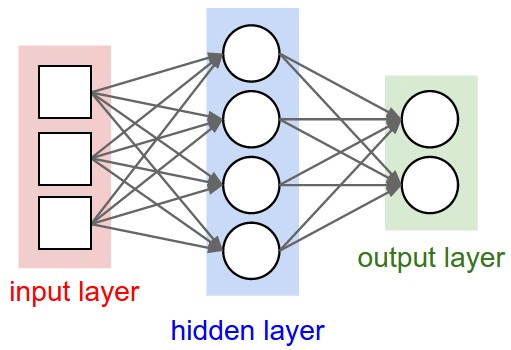
\includegraphics[width=0.8\textwidth, height=0.6\textheight]{Images/AIML_MLP_IMG1.jpg}
\end{columns}
\end{frame}


\begin{frame}{ Comparison of Single and 
	\\ Multi Layer Perceptron }
\begin{columns}
\column{0.5\textwidth}
\alert{Single Layer Perceptron}
\begin{itemize}
  \item Does not contain any hidden layer.
  \item Input and output are linked with each other.
  \item Can easily separate two classes.
\end{itemize}
\column {0.5\textwidth}
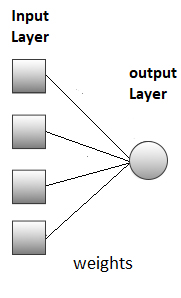
\includegraphics[width=0.8\textwidth, height=0.6\textheight]{Images/AIML_MLP_IMG2.jpg}
\end{columns}
\end{frame}

\begin{frame}{ Comparison of Single and 
	\\ Multi Layer Perceptron }
\begin{columns}
\column{0.5\textwidth}
\alert{Multi Layer Perceptron}
\begin{itemize}
  \item Contains one or more hidden layers.
  \item There are multiple layers between input and output layers which are known as hidden layers.
  \item Can solve complex problems.
\end{itemize}
\column {0.5\textwidth}
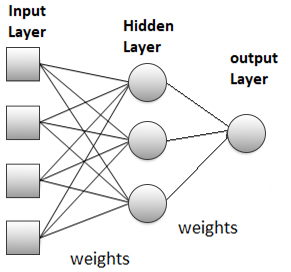
\includegraphics[width=0.8\textwidth, height=0.6\textheight]{Images/AIML_MLP_IMG3.jpg}
\end{columns}
\end{frame}

\begin{frame}{Multi Layer Perceptron}
\begin{itemize}
\item MLP consists of at least three layers: \\
\begin{itemize} \item input layer
		\item  output layer
		\item  hidden layer
\end{itemize}
\item First layer is the input and the last layer is the output.
\item If there is more than one hidden layer, we call them “deep” neural networks.
\item Except for the input layer, each layer uses a nonlinear activation function (Eg. Sigmoid function).
\end{itemize}
\end{frame}

\begin{frame}{Matrix Multiplication}
\begin{columns}
\column{0.5\textwidth}	
\begin{itemize}
  \item Considering input layer, hidden layer and output layer
  \item {$inputs = \begin{bmatrix} x_1 \\ x_2 \\ x_3 \\ x_4 \end{bmatrix} $}
  \item {$Input weights = \begin{bmatrix}w_{1} & w_{2} & w_{3} & w_{4} \\ w_{5} & w_{6} & w_{7} & w_{8} \\ w_{9} & w_{10} & w_{11} & w_{12} \\
                          \end{bmatrix}$}
  
\end{itemize}
\column {0.5\textwidth}
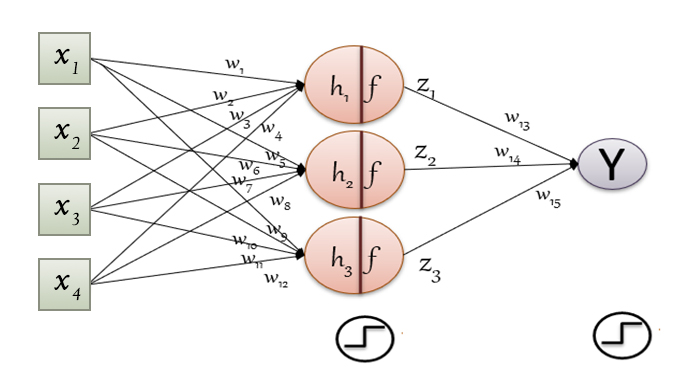
\includegraphics[width=0.8\textwidth, height=0.6\textheight]{Images/AIML_MLP_IMG4.jpg}
\end{columns}
\end{frame}

\begin{frame}{ Matrix Multiplication }
\begin{columns}
\column{0.5\textwidth}	
\begin{itemize}
  \item Perform dot product of inputs and weights, \\
  $w_{1}x_{1} + w_{2}x_{2} + w_{3}x_{3} + w_{4}x_{4}$ \\
  \item Pass the value through the activation function \\
  $Z_{1} = f\left ( \sum_{i=1}^{4} w_{i}x_{i}\right )$ \\
  \item Similarly, calculate Z\_{2} and Z\_{3}
\end{itemize}
\column {0.5\textwidth}
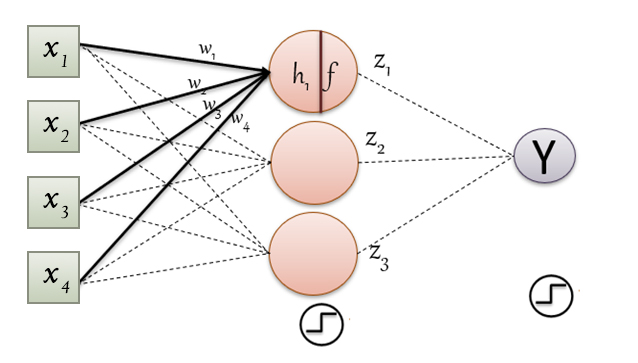
\includegraphics[width=0.8\textwidth, height=0.6\textheight]{Images/AIML_MLP_IMG5.jpg}
\end{columns}
\end{frame}

\begin{frame}{ Matrix Multiplication }
\begin{columns}
\column{0.5\textwidth}	
\begin{itemize}
  \item Outputs of the hidden layer are Z\_{1}, Z\_{2} and Z\_{3} \\
  \item For the final output, perform the dot product of hidden layer outputs and hidden layer weights \\
  \item Pass through the activation function to get the output of the output layer.\\
  	{$ \begin{bmatrix}
 	w_{13} & w_{14} & w_{15} \\
	\end{bmatrix}
	\begin{bmatrix}
 	Z_{1}\\
 	Z_{2}\\
 	Z_{3}
	\end{bmatrix}$}\\
  	Y = {$ f(W_{13}Z_{1} + W_{14}Z_{2} + W_{15}Z_{3} +) $}
            {$ = f\left ( \sum_{j}^{} w_{j}z_{j}\right )$}
  
\end{itemize}
\column {0.5\textwidth}
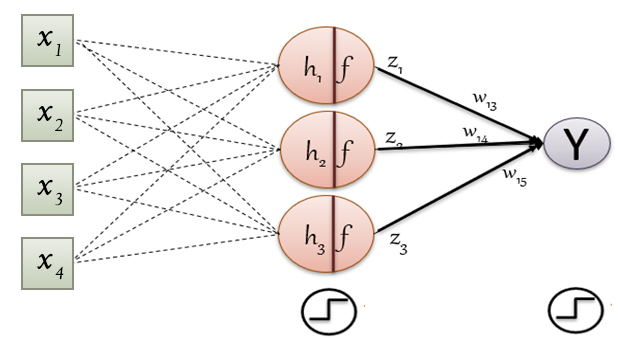
\includegraphics[width=0.8\textwidth, height=0.6\textheight]{Images/AIML_MLP_IMG6.jpg}
\end{columns}
\end{frame}


\begin{frame}{Multiple Layers}
\begin{columns}
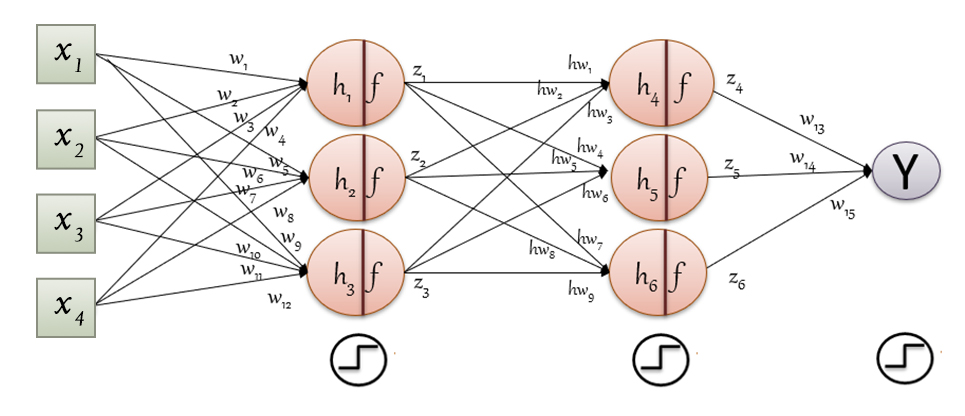
\includegraphics[width=1.0\textwidth, height=0.6\textheight]{Images/AIML_MLP_IMG7.jpg}
\end{columns}
\end{frame}

\begin{frame}{Outlier}
\begin{itemize}
\item Activation function decides whether a neuron should be activated or not. \\
\centering
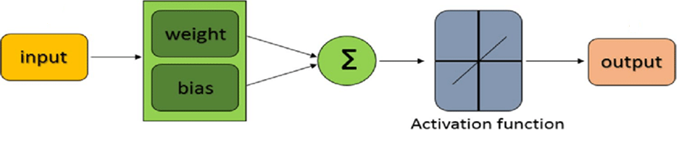
\includegraphics[width=8.5cm , height=3.7cm]{Images/AIML_MLP_IMG8.png}
\end{itemize}
\end{frame}

\begin{frame}{ Classification Problem }
\begin{columns}
\column{0.5\textwidth}
\begin{itemize}
  \item In this problem, we cannot separate classes with a single line.
  \item Requires more than 2 lines for separating the classes.
  \item Single perceptron cannot fully separate the classes. \\
  Whereas Multi-layer perceptron can separate nonlinearly \\
  separable classes using multiple lines.
\end{itemize}
\column {0.5\textwidth}
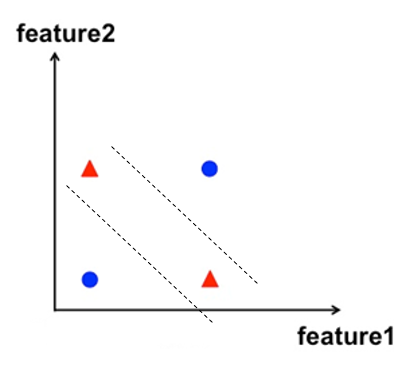
\includegraphics[width=0.5\textwidth, height=0.5\textheight]{Images/AIML_MLP_IMG9.png}
\end{columns}
\end{frame}

\begin{frame}{ Solve Classification Problem }
\begin{columns}
\column{0.5\textwidth}
\begin{itemize}
  \item Draw a decision boundary that splits the two classes.
  \item There is more than one possible decision boundary that splits the data correctly.
  \item Two lines are required to represent the decision boundary.
\end{itemize}
\column {0.5\textwidth}
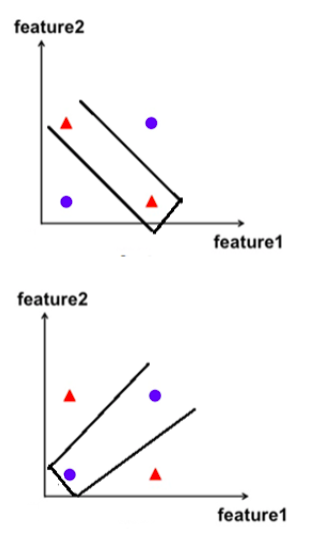
\includegraphics[width=0.9\textwidth, height=0.7\textheight]{Images/AIML_MLP_IMG10.png}
\end{columns}
\end{frame}

\begin{frame}{ Solve Classification Problem }
\begin{figure}
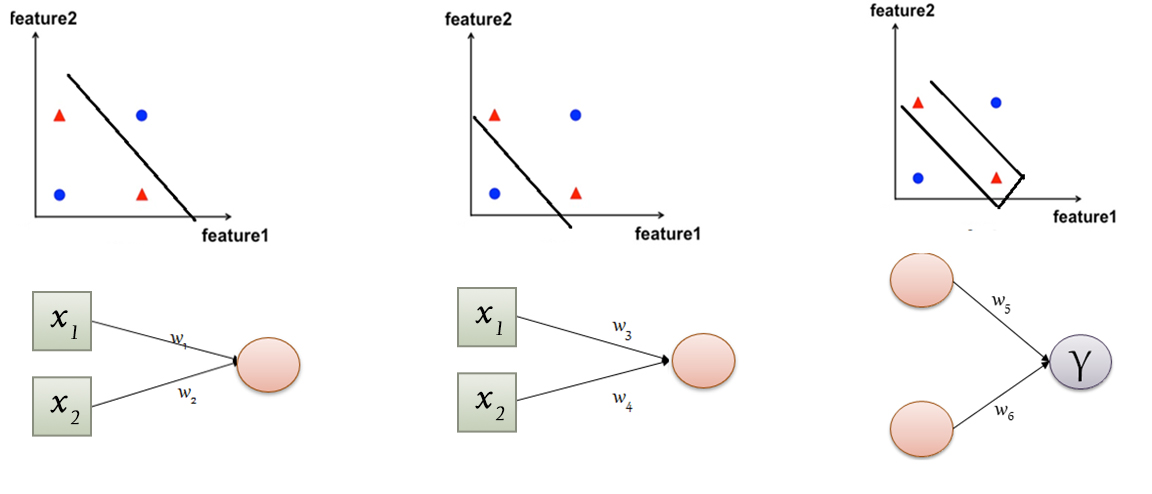
\includegraphics[width=12cm, height=6cm]{Images/AIML_MLP_IMG12.jpg}
\end{figure}
\end{frame}

\begin{frame}{ Solve Classification Problem }
\begin{columns}
\column{0.5\textwidth}
\begin{itemize}
  \item Require only one hidden layer with two hidden neurons.
  \item Outputs of the two hidden neurons are to be merged into a single output.
\end{itemize}
\column {0.5\textwidth}
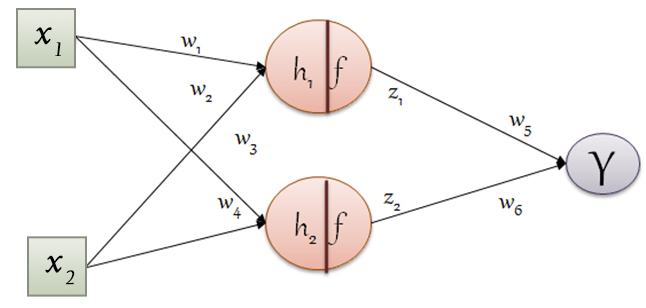
\includegraphics[width=0.6\textwidth, height=0.3\textheight]{Images/AIML_MLP_IMG13.jpg}
\end{columns}
\end{frame}

\begin{frame}{Demo Experiments}
\alert{Code Available}
\begin{itemize}
\item {Demo1}
	\begin{itemize}
		\item Classify non-separable data using MLP Classifier
	\end{itemize}
\item {Demo2}
	\begin{itemize}
		\item Solving Complex equations using MLP Regressor
	\end{itemize}
\end{itemize}
\end{frame}

\begin{frame}{ Summary }
\begin{columns}
\column{1.0\textwidth}
\begin{itemize}
  \item A Multi-Layer Perceptron (MLP) contains one or more hidden layers (apart from one input and one output layer).
  \item Multiple layers and non-linear activation distinguish MLP from a linear perceptron.
\end{itemize}
\column {1.0\textwidth}
\end{columns}
\end{frame}

\begin{frame}{ Terminology }
\begin{columns}
\column{1.0\textwidth}
\begin{itemize}
  \item Neuron
  \item Weights
  \item Perceptron
  \item Hidden Layer
  \item Activation Function
  \item Multi-layer Perceptron
\end{itemize}
\column {1.0\textwidth}
\end{columns}
\end{frame}



{ \1
\begin{frame}
	\title{Thanks!!}
	\subtitle{Questions?}
	\maketitle
\end{frame}
}

\end{document}
